\documentclass[xetex,final,10pt]{beamer}

% 8em ~ 12cm
% 1cm ~ 0.66em

\usetheme{I6dv}

\usepackage{type1cm}
\usepackage{calc}
\usepackage{times}
\usepackage{amsmath,amsthm, amssymb, latexsym}
\usepackage{fontspec}
\usepackage{xunicode} %Unicode extras!
\usepackage{xltxtra}  %Fixes
\usepackage{tikz}
\usepackage{tikz-bpmn}
\usepackage{enumitem}
\usepackage{ragged2e}
\usepackage{rotating}
\usepackage{relsize}
\usepackage{setspace}
\usepackage{hyperref}
\definecolor{light-gray}{gray}{0.97}
\usepackage{listings}
\usepackage{listings-C}
\usepackage{listings-modernC}
\lstloadlanguages{C11,C99}
\lstset{
language=[errnoPOSIX]{C},
language=[tgmath]{C},
language=[threads]{C},
language=[stdatomic]{C},
language=[boundschecking]{C},
language=[99]{C},
language={C11},
style=modernC,
basicstyle=\tt\normalsize,
moreemph=[5]{
futex_wait,
futex_wake,
},
moreemph=[3]{
smpl_lock,
smpl_unlock,
smpl, ftx,
ftx_bit,
ftx_fetch_add,
ftx_cmpxch,
ftx_load,
ftx_lock,
ftx_unlock,
ftx_mask,
ftx_count,
ftx_set,
ftx_lkd,
ftx_contrib,
},
numbers=none,
}

\newcommand{\titleone}[1]{\fontsize{1.75cm}{1em}\selectfont#1}

\newcommand{\mojtitle}{%
    \titleone{%
      Futex based locks for C11's generic atomics}
  }


\usetikzlibrary{positioning,calc,fit}
\boldmath
\usepackage[english]{babel}
\usepackage[orientation=portrait,size=A1]{beamerposter}
\setbeamersize{text margin left=30mm}
\setbeamersize{text margin right=30mm}
\title{Futex based locks for C11's generic atomics}
\author{Jens Gustedt}
\institute{INRIA}

\tikzstyle{every picture}=[line width=1.2pt]

\setbeamertemplate{itemize items}[circle]
\setbeamerfont{itemize/enumerate subbody}{size=\normalsize}
\setbeamerfont{itemize/enumerate subsubbody}{size=\normalsize}

\newcommand{\bigme}[2]{{\normalsize\raisebox{#1}{#2}}}
\newcommand{\fat}[1]{\textbf{#1}}

\setsansfont[
 Path=fonts/,
 BoldFont={Aller_Bd.ttf},
 ItalicFont={Aller_It.ttf},
 BoldItalicFont={Aller_BdIt.ttf}
 ]{Aller_Rg.ttf}

\setmonofont[Path=fonts/,Scale=0.9]{VeraMono.ttf}

\setlist[itemize,1]{itemsep=0.5ex,leftmargin=2.5em,itemindent=0em,labelsep=0.3em,
      label=\scalebox{1.0}{\textbullet},
      after=\vspace{.25\baselineskip},before=\vspace{.25\baselineskip}}

\setlist[itemize,2]{leftmargin=1.5em,label=-}

\setlist[description]{itemsep=0.5ex,leftmargin=2.5em,itemindent=0em,labelsep=0.3em}

\begin{document}%
\pgfdeclarelayer{backg}%
\pgfsetlayers{backg,main}
%
    \begin{frame}[fragile]%
    \small% TODO
%
% BACKGROUND
%
\begin{tikzpicture}[remember picture,overlay]%
    \node [xshift=-18em,yshift=1em] at (current page.south west) {
        \begin{tikzpicture}[remember picture,overlay,scale=5,opacity=0.4]
            \foreach \i in {1,1.5,...,50}
                \draw[white,line width=0.15em] (0, {2*\i}) -- ({100/\i}, 0);
        \end{tikzpicture}
    };
\end{tikzpicture}%
%
\begin{tikzpicture}[remember picture,overlay]%
    \node [xshift=24em,yshift=5em] at (current page.north east) {
        \begin{tikzpicture}[remember picture,overlay,scale=5,opacity=0.4]
            \foreach \i in {1,1.5,...,50}
                \draw[white,line width=0.15em] (0, {-2*\i}) -- (-{100/\i}, 0);
        \end{tikzpicture}
    };
\end{tikzpicture}%
%
\begin{tikzpicture}[remember picture,overlay]%
    \node(headline) [xshift=0em,yshift=-1.5em,align=center,white,text width=\paperwidth,
             fill=i6colorblockbg] at (current page.north) {
        \\[11.5em]
        \usebeamercolor{title in headline}{
            \color{white} % fg
            \begin{minipage}{\textwidth}
                \begin{center}
                \ \\[1.8em]
                {\Huge\bfseries\mojtitle }\\[1em]
                {\huge{}Jens Gustedt}\\[0.7em]
                {\large{}\href{mailto:jens.gustedt@inria.fr}{jens.gustedt@inria.fr}}\\[0.9em]
                {\LARGE{}INRIA, ICube, Université de Strasbourg}
                \end{center}
            \end{minipage}
            \ \\[1.5em]
        }
    };
    \draw[line width=0.15em,lighthead] (headline.south west) -- (headline.south east);
\end{tikzpicture}%
%
\vskip 16em
\newcommand{\odstep}{\vskip 8ex}

\begin{center}
    \begin{columns}[t]
        \begin{column}{0.48\textwidth}
            \begin{block}{\bigme{0em}{Tools for data consistency and
                  races: {\color{red}Atomics}}%
            \\[-1.1em]}

          \begin{itemize}
          \item {\color{red}Atomic instructions} are present in all modern processors.
          \item They are the basis of all thread level parallelism:
            \begin{itemize}
            \item Schedule concurrent tasks.
            \item Deal with concurent data access.
            \end{itemize}
          \item C11 introduced atomic data types and operations.
          \item If atomics for a particular have no hardware support:
            \begin{itemize}
            \item generic atomics
            \end{itemize}
          \item ... {\color{red}need an efficient OS-supported lock.}
          \end{itemize}


            \end{block}
            \odstep

            \begin{block}{\bigme{0em}{Tools for data consistency and
                  races: {\color{red}\texttt{futex}}}%
            \\[-1.1em]}

          \begin{itemize}
          \item In addition to atomics, and OS needs an efficient tool
            to have threads wait (sleep).
          \item Linux has {\color{red}\texttt{futex}}.
          \item Combines atomic data and an OS wait queue.
            \begin{itemize}
            \item \lstinline{futex_wait} guarantees that the value of the
              lock is what we think
            \item \lstinline{futex_wake} can wake up one or several threads
            \end{itemize}
          \end{itemize}


            \end{block}
            \odstep

\begin{block}{\bigme{-3pt}{A new generic lock algorithm using futex system calls}\\[-0.9em]}

  \begin{itemize}
  \item ideas:
    \begin{itemize}
    \item combine lock and wait counter in one atomic data
    \item count the right thing
      \begin{itemize}
      \item number of threads inside critical section
      \item not only those inside \lstinline{futex_wait}
      \end{itemize}
    \item do \emph{some} active spinning before going into
      \lstinline{futex_wait}
    \item but not too much.
    \end{itemize}
  \item reduces the number of synchronous memory operations and bandwidth
  \item can be proven to be deadlock free
  \end{itemize}
\end{block}
\odstep

\newcommand{\solucja}[2]{%
    \href{#2}{\textbf{#1}}}

\begin{block}{
    \bigme{3pt}
    {Benchmarks}
    %\\[-0.9em]
  }
  Benchmark a \emph{\color{red}worst case} code for locks:
  \begin{itemize}
  \item High frequency update of a dynamic data structure.
  \item High load with a lot of threads.
  \item High probability of failure for the access.
  \end{itemize}

  Put the system under \emph{\color{red}heavy stress.}\\[2ex]

  Platform:
  \begin{itemize}
  \item a 4 core ARM
  \item Alpine Linux\hfill \url{https://www.alpinelinux.org/}
  \item based on \texttt{musl}\hfill http://www.musl-libc.org/
  \end{itemize}


\end{block}
\odstep

\newcommand{\litera}[1]{\makebox[1em][c]{(#1)}}

\begin{block}{
    \bigme{3pt}{Analysis}%
    %\\[-0.9em]
  }

  Good combination of
  \begin{itemize}
  \item spinlock stragegy for few congestions
  \item OS wait strategy for congestion
  \end{itemize}


  Outperforms native approaches

  \begin{itemize}
  \item \texttt{Gcc} builtin strategy
  \item native mutex
  \item \texttt{musl}'s internal lock
  \end{itemize}
\end{block}
\odstep

\begin{block}{Perspective}
  Integrate the new strategy in \texttt{musl}
\end{block}

\odstep

\newcommand{\cimark}[2]{[\href{#2}{#1}]}

\newcommand{\bink}[2]{%
    \href{#2}{\normalsize{}[ {#1}\:]}\quad%
}

        \end{column}
        \begin{column}{0.48\textwidth}

\newsavebox\blockbox
\newenvironment{myblock}{%
  \begin{lrbox}{\blockbox}%

    \begin{minipage}{.95\textwidth}
}{
    \end{minipage}
  \end{lrbox}
  \tikz\node[
    fill=white,
    draw=lighthead,
    line width=3pt,
    inner sep=15pt,
    outer sep=0pt,
  ]{\usebox\blockbox};
}

\newcommand{\skipper}{\vskip 1em}

\begin{myblock}{A simple \texttt{futex}-based lock.}
\begin{lstlisting}
typedef _Atomic(int) smpl;
void smpl_lock(smpl* lck) {
 for (;;) {
  int prev = atomic_exchange(lck, 1);
  if (!prev) break;
  futex_wait(lck, prev);
 }
}
void smpl_unlock(smpl* lck) {
 atomic_store(lck, 0);
 futex_wake(lck, 1);
}
\end{lstlisting}
\end{myblock}
\skipper

\begin{myblock}{The new counter based locking strategy}
\begin{lstlisting}
typedef _Atomic(unsigned) ftx;
#define ftx_set(VAL)  (0x80000000u | (VAL))
#define ftx_lkd(VAL)  (0x80000000u & (VAL))

void ftx_lock(ftx* lck) {
 unsigned cur = 0;
 if (!ftx_cmpxch(lck, &cur, ftx_set(1))) {
  cur = ftx_fetch_add(lck, 1) + 1;
  for (;;) {
   while (!ftx_lkd(cur)) {
    if (ftx_cmpxch(lck, &cur, ftx_set(cur))) return;
    for (unsigned i = 0; i < E && ftx_lkd(cur); i++)
     cur = ftx_load(lck);
   }
   while (ftx_lkd(cur)) {
    futex_wait(lck, cur);
    cur = ftx_load(lck);
   }
  }
 }
}
\end{lstlisting}
\end{myblock}
\skipper

\begin{myblock}{lock throughput on an ARM platform}
\begin{center}
  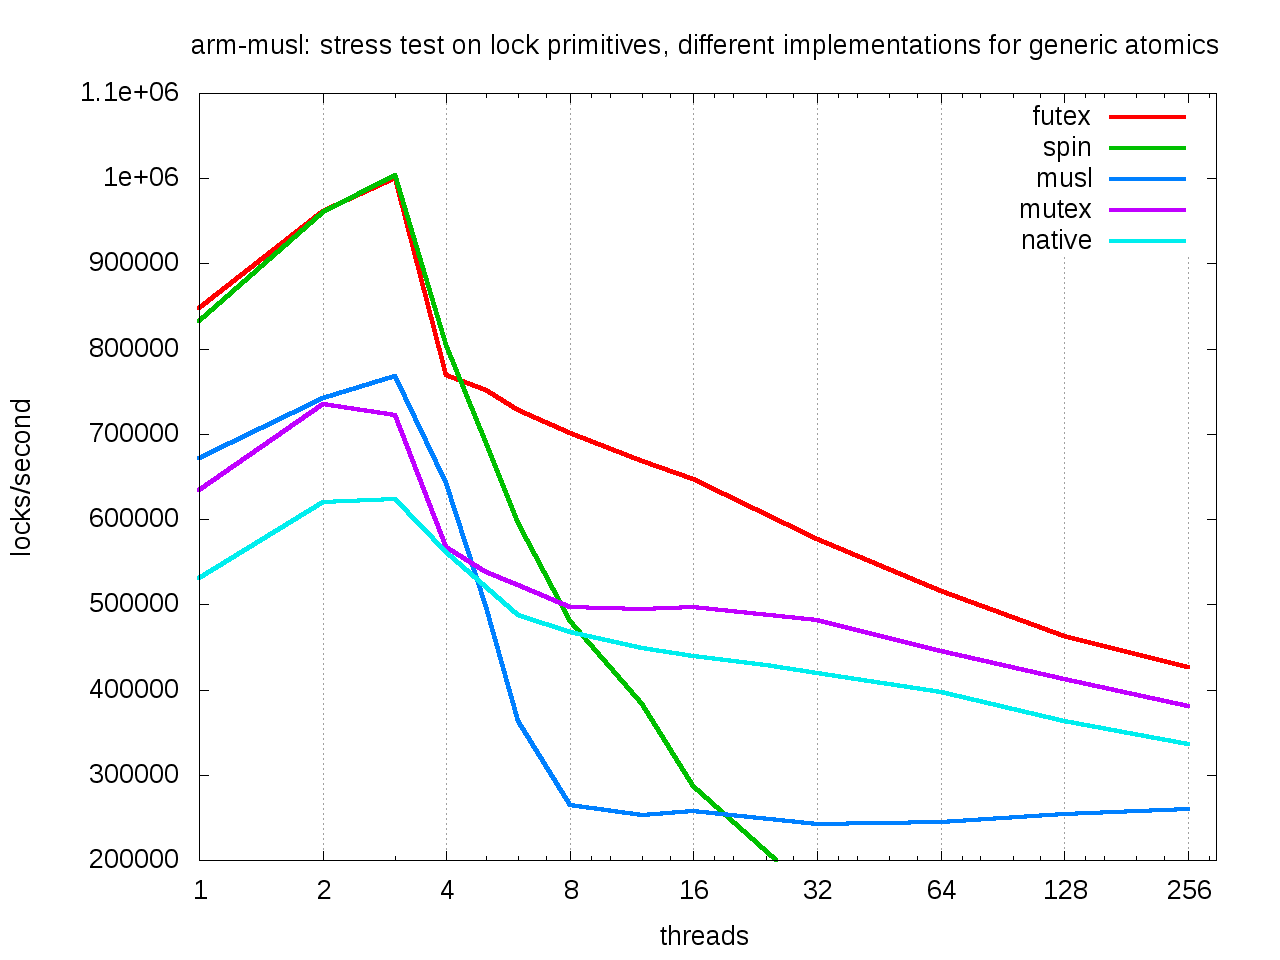
\includegraphics[width=0.65\textwidth]{../benchs/arm/test-arm-u64.png}
\end{center}\vskip 0.7em
\end{myblock}
\skipper

\begin{myblock}{Relative performance}
\begin{center}
  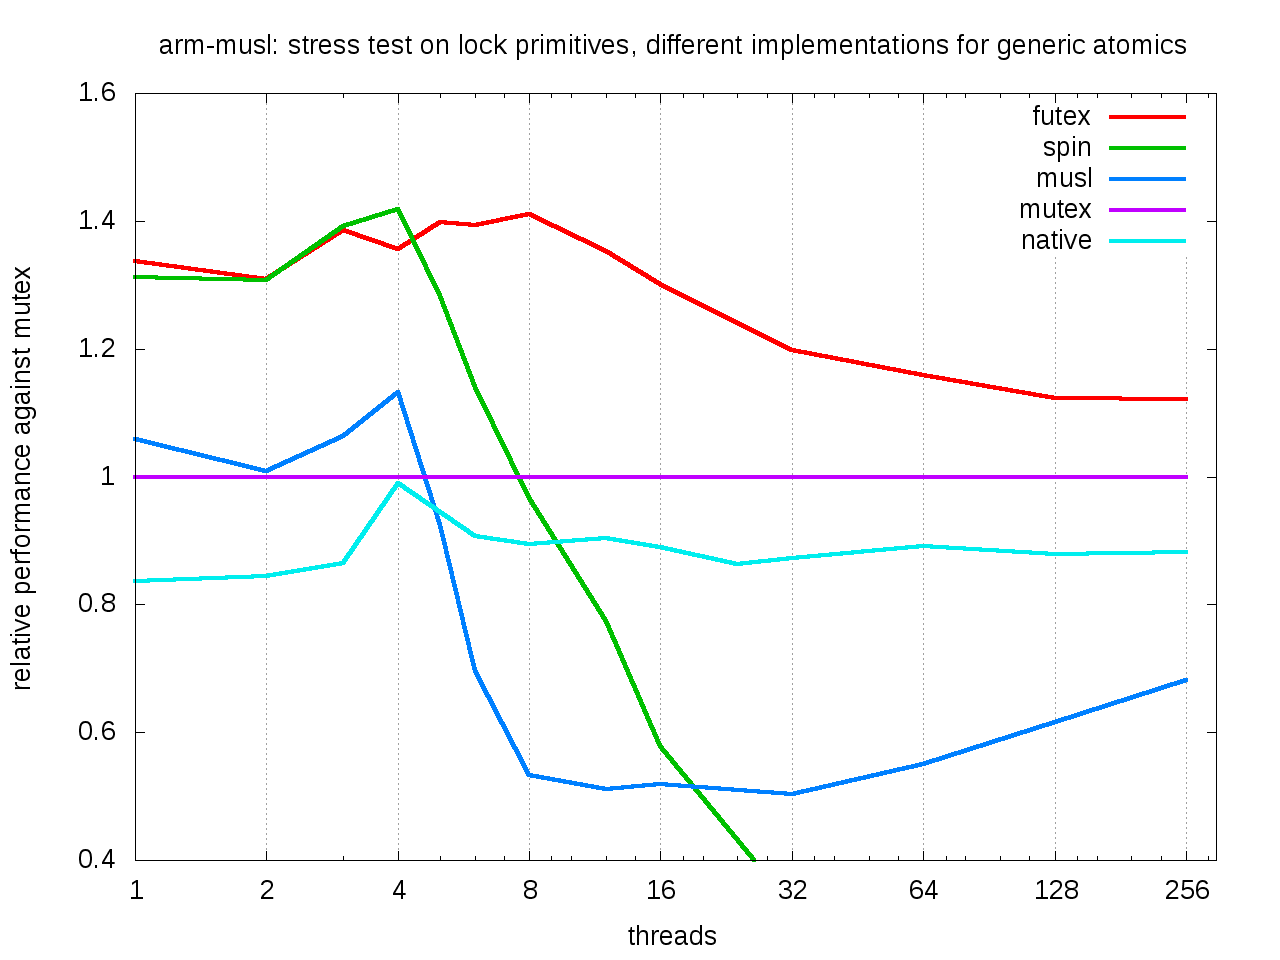
\includegraphics[width=0.65\textwidth]{../benchs/arm/test-arm-u64-relative.png}
\end{center}\vskip 0.7em
\end{myblock}
\skipper


        \end{column}

    \end{columns}
\end{center}
\end{frame}

\end{document}
